\section{Resultados}

% \textsl{En esta secci\'on presentaremos los resultados obtenidos 
% al utilizar diferentes trazas.}

\vspace*{0.3cm}

\subsection{Trazas utilizadas}

Las trazas que utilizamos fueron las generadas utilizando la
clase \texttt{MainTraceGenerator.java} provista por la cátedra,
y dos generadas por nosotros, estas son:

\begin{itemize}
    \item
            \textbf{Random0}
            Se ejecuta dos veces una transacci\'on sobre 100 bloques
            distintos en una tabla de 200 bloques.
            
    \item
            \textbf{Random1}
            Se realizan 1000 accesos random a una tabla de 200 bloques.

\end{itemize}

Dichas trazas pueden encontrarse en la carpeta 
\texttt{ubadb/generated}.


\subsection{Generación de resultados}

Modificamos la clase \texttt{MainEvaluator} para ofrecer la opción de
evaluar una traza dada utilizando \texttt{SingleBufferPool}
y \texttt{MultipleBufferPool}. 

\vspace*{0.5cm}

Creamos la clase \texttt{TpEvaluator}, ubicada en
\texttt{core/external/bufferManagement}, que lo que hace es
correr sets de trazas y evaluarlas usando \texttt{SingleBufferPool}
y \texttt{MultipleBufferPool}

\begin{verbatimtab}[4]
public class TpEvaluator 
{
	static PageReplacementStrategy pageReplacementStrategy;
	pageReplacementStrategy = new FIFOReplacementStrategy();

	public static void main(String[] args)
	{
		runBNLJTraces();
		runFileScanTraces();
		runIndexScanTraces();		
		runRandomTraces();
	}

	...
}
\end{verbatimtab}

Cada función \texttt{runXTraces} crea una lista con los nombres de las trazas
correspondientes y se lo pasa a la función \texttt{runTraces}.
Por ejemplo, para el caso de \texttt{indexScan} se realiza lo siguiente

\newpage

\vspace*{-0.2cm}

\begin{verbatimtab}[4]
private static void runIndexScanTraces()
{
	List<String> traceFileNames = new LinkedList<String>();
	
	/* Index Scan. */
	traceFileNames.add("generated/indexScanClustered-Product.trace");
	traceFileNames.add("generated/indexScanClustered-Sale.trace");
	traceFileNames.add("generated/indexScanUnclustered-Product.trace");
	traceFileNames.add("generated/indexScanUnclustered-Sale.trace");
	
	System.out.println("\nIndex Scan\n");		
	runTraces(traceFileNames);
}
\end{verbatimtab}

\texttt{runTraces} toma una lista de nombres de trazas y para cada una llama
a las funciones correspondientes para evaluarla usando Single y Multiple buffer pools.

\begin{verbatimtab}[4]
private static void runTraces(List<String> traceFileNames)
{
	for (String traceFileName: traceFileNames)
	{
		try
		{				
			System.out.println("\nTrace: " + traceFileName);
			evaluateWithSingle(traceFileName);
			evaluateWithMultiple(traceFileName);
		}
		catch(Exception e)
		{
			System.out.println("FATAL ERROR (" + e.getMessage() + ")");
			e.printStackTrace();
		}
	}
}
\end{verbatimtab}

\texttt{evaluateWithSingle} toma diferentes tamaños de buffer, y para
cada uno, evalúa la traza, llamando a la función correspondiente
de \texttt{MainEvaluator}.

\newpage

\texttt{evaluateWithMultiple} lee diferentes catálogos, previamente
creados, que puden encontrarse en \texttt{ubadb/catalogs}. 
Cada uno de ellos tiene los buffers \texttt{Default, Keep, Recycle}
con tamaños que van variando.

\vspace*{0.5cm}

Tenemos cuatro grupos de catálogos, dentro de cada grupo hay 7 
catálogos de diferentes tamaños.

\begin{enumerate}
	\item
		\textbf{equal\_size}
		todos los buffers tienen el mismo tamaño, que se corresponde
		con el de single.
		
	\item
		\textbf{bigger\_default}
		\texttt{Keep} y \texttt{Recycle} tienen el mismo tamaño, 
		que es el que se corresponde con el de single, y 
		\texttt{Default} tiene el doble de tamaño.

	\item
		\textbf{bigger\_keep}
		\texttt{Default} y \texttt{Recycle} tienen el mismo tamaño, 
		que es el que se corresponde con el de single, y 
		\texttt{Keep} tiene el doble de tamaño.

	\item
		\textbf{bigger\_recycle}
		\texttt{Keep} y \texttt{Default} tienen el mismo tamaño, 
		que es el que se corresponde con el de single, y 
		\texttt{Recycle} tiene el doble de tamaño.
\end{enumerate}

Para la asignación en buffer, pusimos una tabla en cada uno de los
buffers.

\vspace*{0.5cm}

Para cada caso, se evalúa la traza, llamando a la función correspondiente
de \texttt{MainEvaluator} y se muestra el hit rate obtenido.

\vspace*{0.5cm}

Para las trazas de \texttt{BNLJ} tuvimos en cuenta solamente tamaños
de buffer que fueran grandes, porque si no teníamos un problema de
que no nos alcanzaba la memoria para todos los pedidos.
En el resto de los casos, usamos tanto los tamaños chicos como los
grandes.

\begin{verbatimtab}[4]
private static void evaluateWithSingle(String traceFileName) 
	throws InterruptedException, BufferManagerException, Exception
{
	/* Para BNLJ. */ //int sizes[] = {252, 300, 500, 700}; 
	int sizes[] = {10, 20, 60, 120, 252, 300, 500, 700};
	System.out.println("\nSingleBufferPool\n");
	
	for (int size : sizes)
	{		
		System.out.print(size + " ");
		MainEvaluator.evaluateSingle(pageReplacementStrategy, traceFileName, size);			
	}
}
\end{verbatimtab}

\newpage
\begin{verbatimtab}[4]
private static void evaluateWithMultiple(String traceFileName) 
	throws InterruptedException, BufferManagerException, Exception
{	
	System.out.println("\nMultipleBufferPool");
		
	System.out.println("\nequal_size\n");
	String filename = "catalogs/equal_size/catalog_equal_size_";
	evaluateWithMultipleUsingCatalog(traceFileName, filename);
		
	System.out.println("\nbigger_default\n");
	filename = "catalogs/bigger_default/catalog_bigger_default_";
	evaluateWithMultipleUsingCatalog(traceFileName, filename);
		
	System.out.println("\nbigger_keep\n");
	filename = "catalogs/bigger_keep/catalog_bigger_keep_";
	evaluateWithMultipleUsingCatalog(traceFileName, filename);
		
	System.out.println("\nbigger_recycle\n");
	filename = "catalogs/bigger_recycle/catalog_bigger_recycle_";
	evaluateWithMultipleUsingCatalog(traceFileName, filename);
}
	
private static void evaluateWithMultipleUsingCatalog
	(String traceFileName, String catalogName) 
	throws InterruptedException, BufferManagerException, Exception
{
	for (int i = 0; i < 8; i++)
	//for (int i = 4; i < 8; i++)
	{
		String filename = catalogName + i + ".xml";
		CatalogManager catalogManager = new CatalogManagerImpl("", filename);
		catalogManager.loadCatalog();

		MainEvaluator.evaluateMultiple
			(pageReplacementStrategy, traceFileName, catalogManager);
		}
	}
\end{verbatimtab}


Los resultados obtenidos pueden encontrarse en \texttt{ubadb/results}


\subsection{Resultados obtenidos}

Los casos en los que el touch touch fue 0 se obviaron ya que no 
aportaban para poder realizar comparaciones.

Se encajo una curva a todos los puntos a la vez, esto nos deja ver
el ``caso promedio'', y teniendo esto en cuenta podemos saber en 
qué casos se mejora la performance y en qué casos no.

\begin{figure}[H] \centering
    \subfloat[Random0]
    {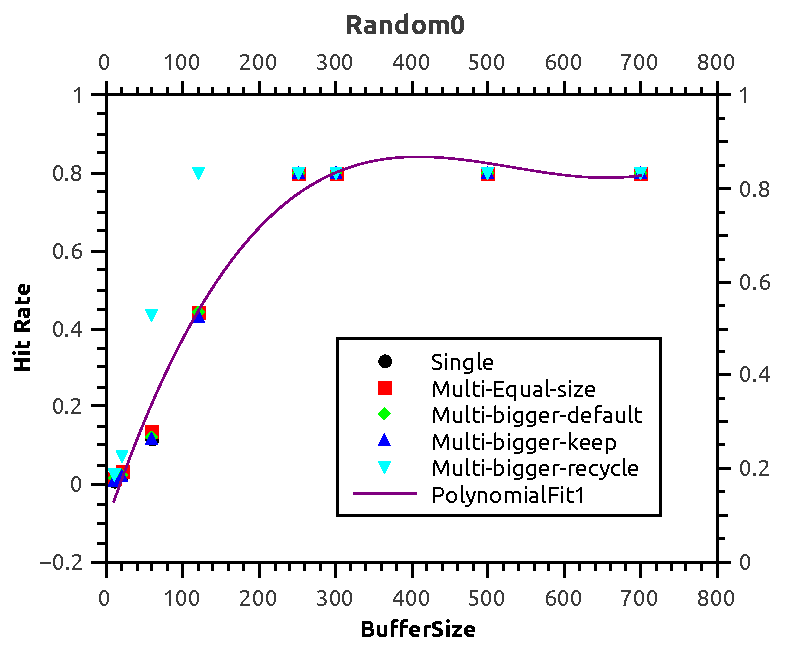
\includegraphics[scale = 0.7]{./img/Random0.pdf}}
\end{figure} 

\vspace*{0.3cm}

\begin{figure}[H] \centering
    \subfloat[Random1]
    {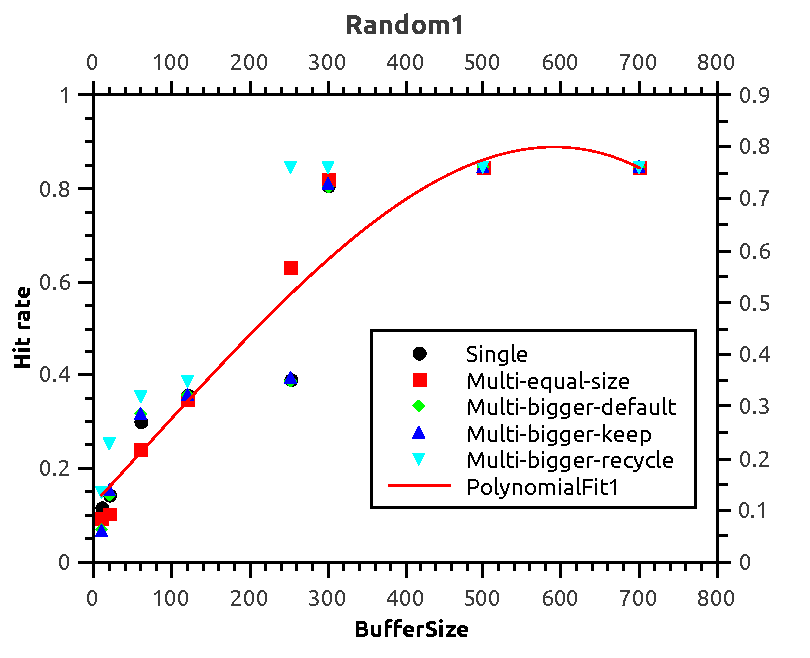
\includegraphics[scale = 0.7]{./img/Random1.pdf}}
\end{figure} 

\begin{figure}[H] \centering
    \subfloat[BNLJ-SaleXProduct-group\_100]
    {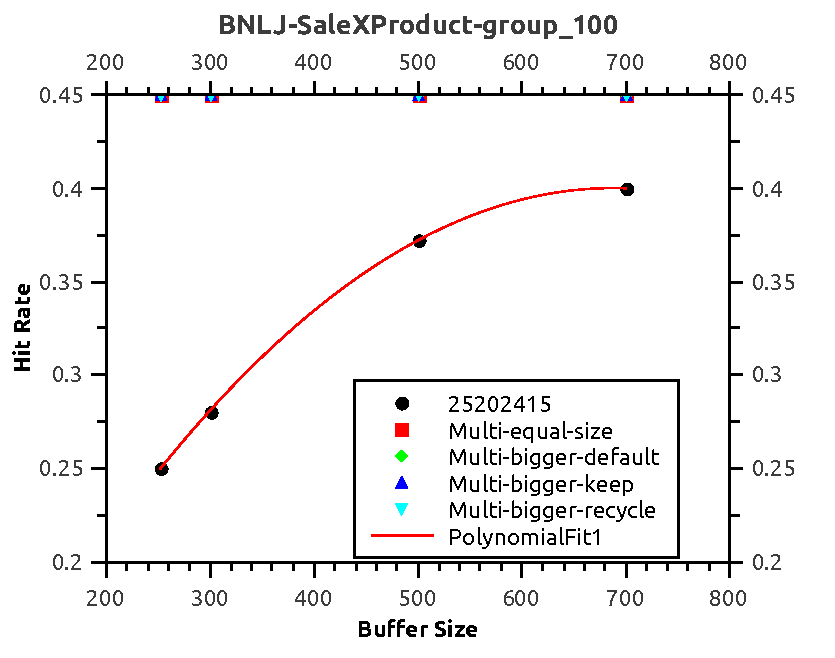
\includegraphics[scale = 0.7]{./img/BNLJ-SaleXProduct-group_100_g.pdf}}
\end{figure}

%\begin{figure}[H] \centering
    %\subfloat[indexScanUnclustered-Product]
    %{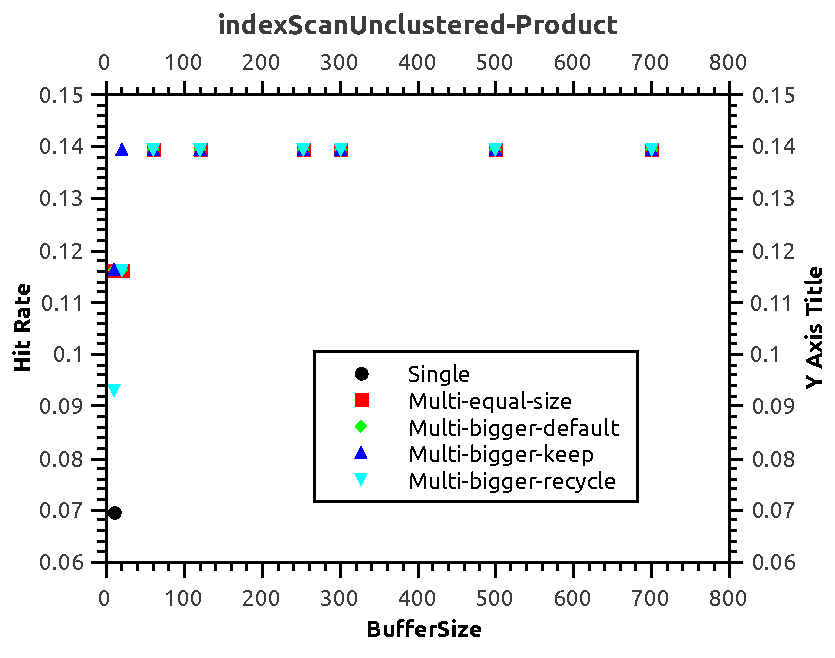
\includegraphics[scale = 0.8]{./img/indexScanUnclustered-Product_g.pdf}}
%\end{figure}

\vspace*{0.5cm}

\begin{figure}[H] \centering
    \subfloat[indexScanUnclustered-Sale]
    {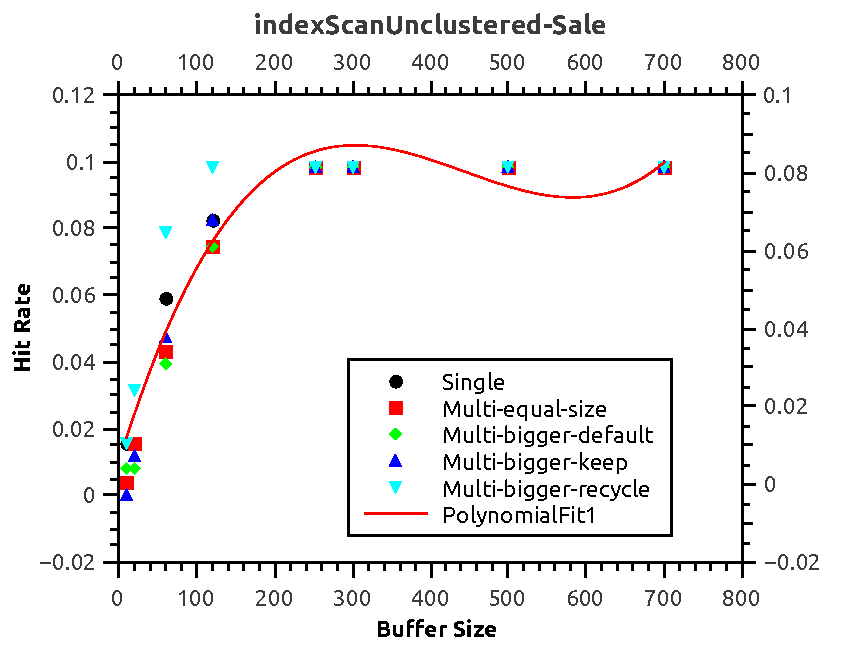
\includegraphics[scale = 0.7]{./img/indexScanUnclustered-Sale_g.pdf}}
\end{figure}
